\documentclass[conference]{IEEEtran}
\IEEEoverridecommandlockouts
% The preceding line is only needed to identify funding in the first footnote. If that is unneeded, please comment it out.
\usepackage{cite}
\usepackage{amsmath,amssymb,amsfonts}
\usepackage{algorithmic}
\usepackage{graphicx}
\usepackage{textcomp}
\usepackage{hyperref}
\usepackage{physics}
\usepackage{mathtools}
\usepackage{comment}
\newcommand{\R}{\mathbb{R}}
\newcommand{\Z}{\mathbb{Z}}
\newcommand{\C}{\mathbb{C}}
\newcommand{\Q}{\mathbb{Q}}

\newcommand{\T}{\mathbb{T}}
\newcommand{\p}{\mathcal{P}}
\newcommand{\N}{\mathbb{N}}
\newcommand{\Hilb}{\mathcal{H}}
\newcommand{\Exp}{\mathbb{E}}
\newcommand{\E}{\mathcal{E}}
\newcommand{\w}{\wedge}\usepackage{xcolor}

\DeclarePairedDelimiter\ceil{\lceil}{\rceil}
\DeclarePairedDelimiter\floor{\lfloor}{\rfloor}

\usepackage{braket}

\renewcommand\bra[1]{{\langle{#1}|}}
\makeatletter
\renewcommand\ket[1]{%
  \@ifnextchar\bra{\k@t{#1}\!}{\k@t{#1}}%
}
\newcommand\k@t[1]{{|{#1}\rangle}}
\makeatother

\def\BibTeX{{\rm B\kern-.05em{\sc i\kern-.025em b}\kern-.08em
    T\kern-.1667em\lower.7ex\hbox{E}\kern-.125emX}}
\begin{document}

\title{A specialized bouquet of instruction prefetchers}


\author{\IEEEauthorblockN{Ayush Agarwal\IEEEauthorrefmark{1},
Sankalan Baidya\IEEEauthorrefmark{2} and Soham Joshi\IEEEauthorrefmark{3}}
\IEEEauthorblockA{Department of Computer Science,
IIT Bombay\\
Mumbai, Maharashtra, India\\
Email: \IEEEauthorrefmark{1} ayushagarwal@cse.iitb.ac.in,
\IEEEauthorrefmark{2} somekoln@cse.iitb.ac.in ,
\IEEEauthorrefmark{3} sohamjoshi@cse.iitb.ac.in}}

\maketitle

\begin{abstract}
This work is built upon IPCP 1.0 by Biswa, which uses a bouquet of prefetchers. We are proposing specialized prefetchers for different categories like Graphs, Sat-solvers, SPEC and Server workloads. This is based upon the intuition that different types of traces will follow different types of access patterns. The ideas used in this work have been built upon from various \verb|DPC3| submissions\cite{b1}\cite{b2}\cite{b3}. % Insert some numbers/results here after result analysis is done
\end{abstract}

\begin{IEEEkeywords}
Prefetechers, Computer Architecture, DPC3 
\end{IEEEkeywords}

\section{Introduction}
% Introduce what Hardware prefetchers are
Hardware prefetching is a technique used by computer processors to fetch data from memory (into the cache) before it's actually needed, reducing the time spent waiting for data to arrive. This is achieved by analyzing memory access patterns and predicting which data is likely to be needed next, and fetching it in advance. 

% Introduce what we have done
In this report, we examine how we have explored ideas from the \href{https://dpc3.compas.cs.stonybrook.edu/?final_programs}{DPC3} submissions and beyond in order to improve upon the performance of the \verb|IPCP| prefetcher. Moreover, we will analyse the increase or decrease in performance via various prefetching strategies in the contexts of graph analytics, SAT Solvers, SPEC, and Server Workload traces. All code, traces used to generate results can be found \href{https://github.com/ChopstickAyush/Riscy\_Data\_Prefetching}{here}. We have used the \href{https://github.com/ChampSim/ChampSim}{Champsim} simulator for all data generated in this report.

% Introduce domain specific building
The authors of \cite{b1} have built an IP (instruction pointer) based prefetcher than can predict majority of the access patterns. However, we find that the themes of accuracy and coverage described in \cite{b2} can be extended to \cite{b1} quite easily. As it turns out, \cite{b3} can be integrated with \cite{b1} as well. These changes often work well with some types of traces and don't work with others. We explore these ideas in the sections below. 

\section{Graph Analytics}
Prefetching in the context of graph analytics has posed a significant challenge in recent times. This is because hardware prefetchers are designed to work well with applications that exhibit predictable memory access patterns. However, graph analytics algorithms, which involve traversing large graphs with irregular memory access patterns, pose a challenge for hardware prefetching. The traversal order of a graph is often dependent on the input data, which makes it difficult for a hardware prefetcher to accurately predict which data to prefetch. Additionally, the size of the graphs used in graph analytics can exceed the capacity of the prefetcher's buffer, making it difficult to store enough prefetched data to improve performance. 

\subsection{Our solution}
We observed that the \verb|IPCP| prefetcher does a good job of predicting strides but, it essentially uses a 1-way associative cache whenever IP-stride tables are required. That is, it uses only the generic parameter \verb|IP| for indexing. However, the themes described in \cite{b2} help us here as we can modify these look up tables in order to generalise them to \textit{multi-parameter} look up tables. Analogous to the paper, we use \verb|IP| and \verb|IP + addr| as our indices, and a $k$-way associative cache with \verb|IP| used to hash the sets, with \verb|IP + addr| giving us the tag. However, this approach does not work as well as we thought it would. The results are given in fig. \ref{graph_rel_ipc_ass}.
\begin{figure}
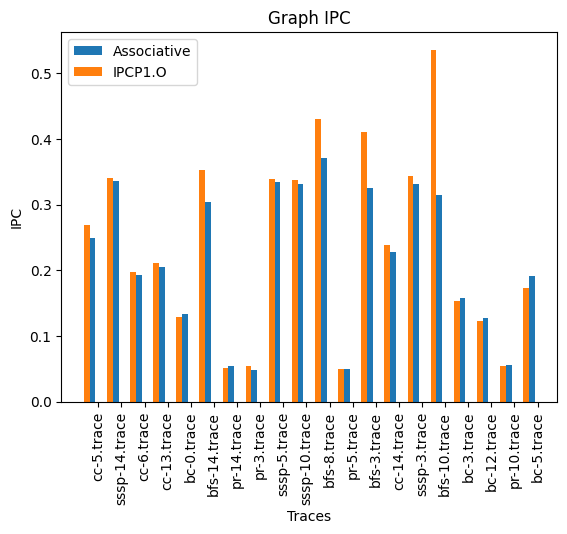
\includegraphics[scale=0.5]{Images/associative.png}
\caption{This figure shows the IPC (instructions per cycle) for IPCP prefetcher, associative table approach, clearly, IPCP is better}
\label{graph_rel_ipc_ass}
\end{figure}

\subsection{A simpler approach}
The previous approach requires making our tables $k$-associative. However, this causes a significant overhead, along with slower look-ups and insertions. Instead of this, we tried simplifying these tables to be 1-way associative, but we use \verb|IP| to index and \verb|IP + addr| to tag, introducing some level of ``specificity". This approach gives us significant performance improvements on graph traces. (ref fig.\ref{graph_rel_ipc}, \ref{graph_ipc}, \ref{graph_l1d}, \ref{graph_l2c})
% add how this is different from using only IP
\begin{figure}
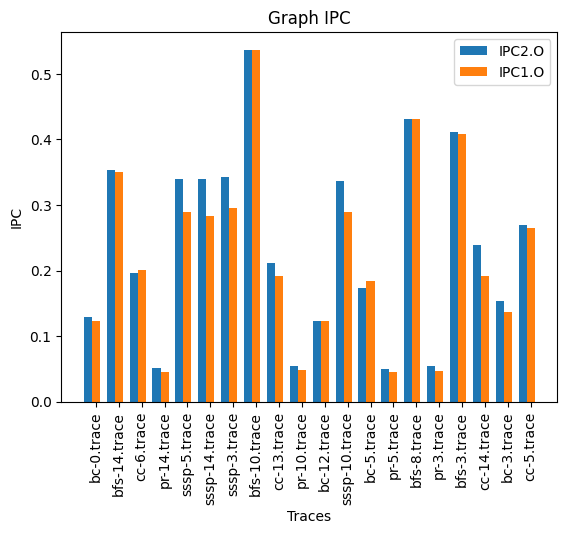
\includegraphics[scale=0.5]{Images/graph_ipc_bar.png}
\caption{This figure shows the IPC (instructions per cycle) for the IPCP prefetcher, when our prefetcher incorporates indexing with IP and tagging via IP and address of the line}
\label{graph_rel_ipc}
\end{figure}
\begin{figure}
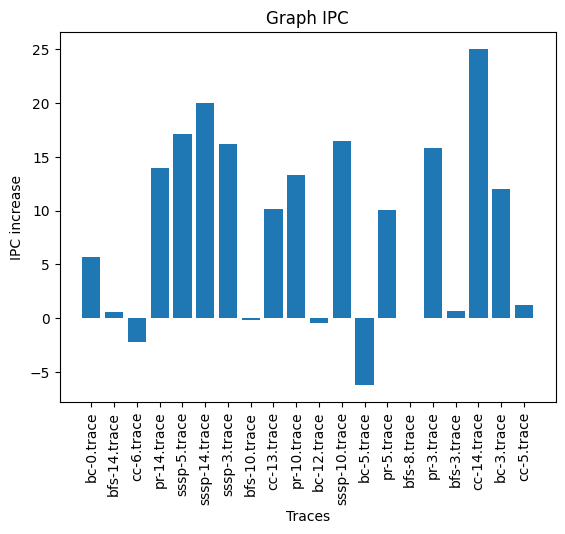
\includegraphics[scale=0.5]{Images/graph_ipc.png}
\caption{This figure shows the IPC (instructions per cycle) relative to the IPCP prefetcher, when our prefetcher incorporates indexing with IP and tagging via IP and address of the line}
\label{graph_ipc}
\end{figure}
\begin{figure}
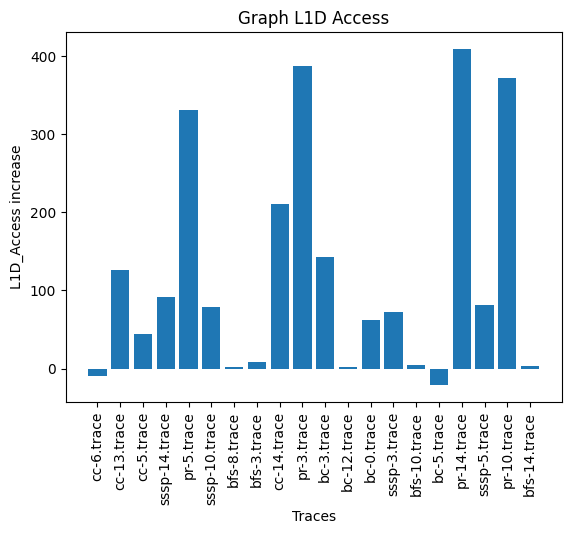
\includegraphics[scale=0.5]{Images/graph_l1d.png}
\caption{This figure shows the Accuracy (hits per accesses) in L1D cache level, relative to the IPCP prefetcher, when our prefetcher incorporates indexing with IP and tagging via IP, address of the line}
\label{graph_l1d}
\end{figure}
\begin{figure}
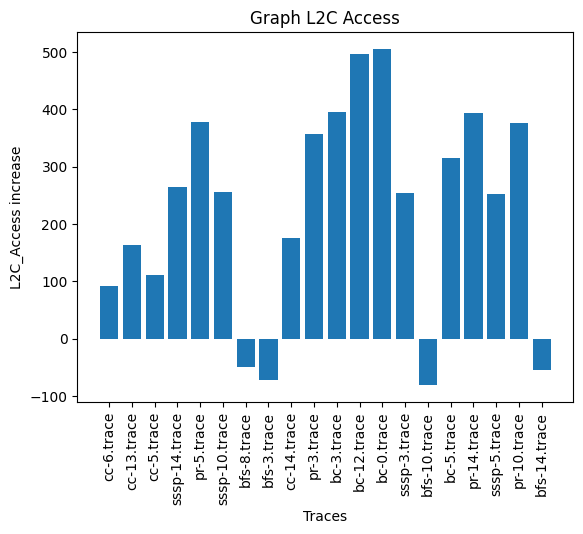
\includegraphics[scale=0.5]{Images/graph_l2c.png}
\caption{This figure shows the Accuracy (hits per accesses) in L2 cache level, relative to the IPCP prefetcher, when our prefetcher incorporates indexing with IP and tagging via IP, address of the line}
\label{graph_l2c}
\end{figure}

\subsection{More specificity in indexing}
We can make the above approach even more specific. Instead of indexing using the \verb|IP|, we now use \verb|IP + addr| for both tagging and indexing. This ofcourse leads to lesser coverage, more accuracy. But, how does this affect our performance metrics? As it turns out, the IPC drops by a significant amount as a consequence of less coverage (even if the IP is same, most of the time, addresses are different). Hence, we have omitted the results for this approach.

\section{SAT Solvers}
Prefetching in this context is again a challenge. This is because hardware prefetching is not effective for SAT solvers because SAT solvers typically access memory in a highly irregular and unpredictable manner. SAT solvers use backtracking search, which requires them to continually traverse different paths in a large search space, making it challenging for a hardware prefetcher to predict which memory locations to prefetch. Additionally, the size of the search space can be quite large, which means that the hardware prefetcher's buffer may not be able to hold enough data to make a significant impact on performance. 

\subsection{Our solution}
Keeping the previous optimisations, we look to build the prefetcher further. First, let's have a look at the results with these optimisations alone. (ref fig. \ref{sat_ipc} \ref{sat_l1d} \ref{sat_l2c}).

\begin{figure}
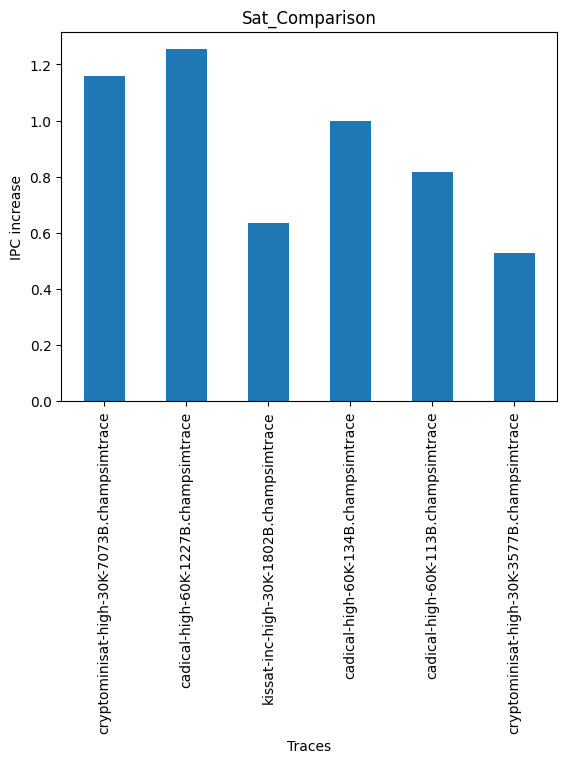
\includegraphics[scale=0.5]{Images/sat_ipc.png}
\caption{This figure shows the IPC (instructions per cycle) relative to the IPCP prefetcher, when our prefetcher incorporates next line prefetcher in LLC}
\label{sat_ipc}
\end{figure}
\begin{figure}
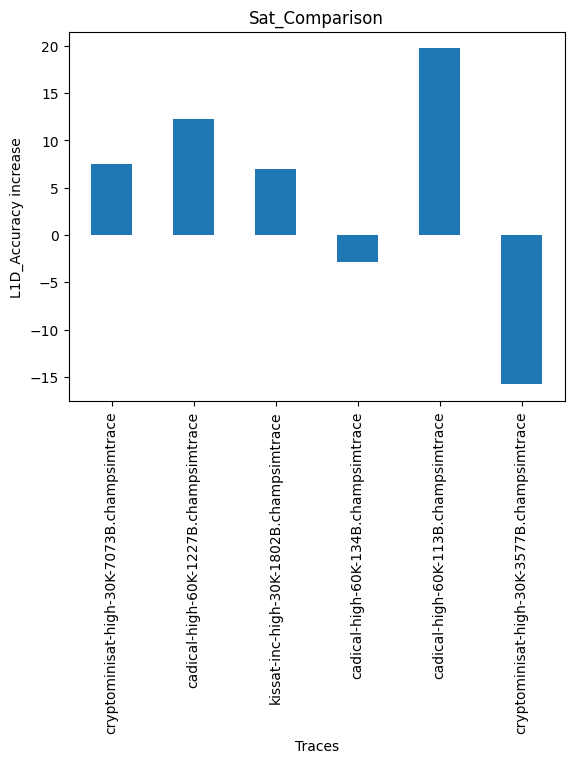
\includegraphics[scale=0.5]{Images/sat_l1d.png}
\caption{This figure shows the Accuracy (hits per accesses) in L1D cache level, relative to the IPCP prefetcher, when our prefetcher incorporates next line prefetcher in LLC}
\label{sat_l1d}
\end{figure}
\begin{figure}
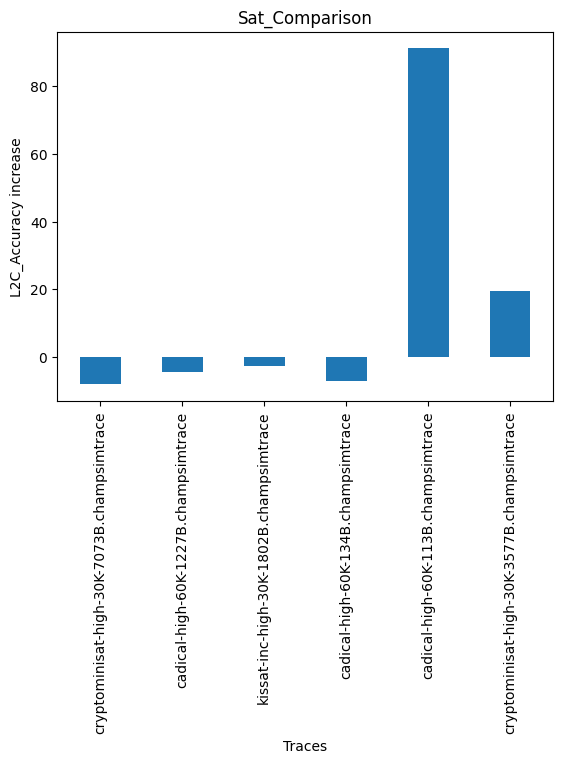
\includegraphics[scale=0.5]{Images/sat_l2c.png}
\caption{This figure shows the Accuracy (hits per accesses) in L2 cache level, relative to the IPCP prefetcher, when our prefetcher incorporates next line prefetcher in LLC}
\label{sat_l2c}
\end{figure}

In order to improve the performance, we turn to \cite{b3}. Since \verb|IPCP| is based upon integrating various stride prefetchers in order predict the next stride correctly, we tried integrating the next line prefetcher into \verb|IPCP|. We have done this at the \verb|LLC| (last-level cache), as that level did not have a prefetcher in the first place. As a result, we observed the following. % Did we integrate mlop in l1d and l2c?

% Insert results here

Since \verb|LLC| has a high size, we can explore putting other prefetching policies in LLC and comparing the results as a scope for further improvement.

\section{SPEC traces}
Why is checking performance on SPEC traces important? This is because the benchmarks developed by SPEC are widely used by industry and academia to measure and compare the performance of different computer systems and components, including processors, memory, storage, and compilers. SPEC benchmarks cover a range of applications and workloads, including scientific and engineering simulations, multimedia processing, and database management.

Let's check the results on SPEC traces with the optimisations done so far.

% Insert results here



\subsection{Our approach}
We need to optimise this further. In order to do so, we tried out the following approach. In order to reduce to losses in SPEC, we observe that replacing \verb|IP + addr| with \verb|IP + cl_addr| helps. Our observations are given below.

% Insert results below


\section{Server Workloads}
Hardware prefetching on server workloads poses a challenge due to reasons quite similar to what we have seen earlier. These workloads often involve a mix of different applications with varying memory access patterns. A hardware prefetcher is designed to predict memory accesses based on a program's access patterns, but in a server environment, applications are frequently switching, making it difficult for the prefetcher to learn the access patterns of each application. Furthermore, server workloads often involve large datasets that can exceed the prefetcher's buffer size, limiting its ability to prefetch data effectively.

Via the current modifications, we observe the following.

% Insert results here.

\subsection{Our approach}
We need to optimise this further. In order to do so, we tried out the following approach. 

% TO BE DONE

\section{Results}
Give a summary of the results here.

\section*{Conclusion and remarks}
This report goes through some optimisations which show a sizeable improvement over the prefetchers presented in DPC3, albeit in application specific traces. The final improvements in IPC are approximately 10\% in graph, 10\% in SAT, 10\% in SPEC and 10\% in Server Workloads. (update actual values later)

\section*{Acknowledgements}
We would like to thank the instructor of CS230, Biswa, for giving us the opportunity to work on this project which allowed us to explore a taste of real-life research. We would also like to thank all the CS230 teaching assistants for solving queries throughout the labs, which in turn allowed us to have sufficient background to work on this project. 

\begin{thebibliography}{00}
\bibitem{b1} S. Pakalapati, B. Panda, ``Bouquet of Instruction Pointers: Instruction Pointer Classifier-based Hardware Prefetching''.
\bibitem{b2} M. Bakhshalipour, M. Shakerinava, P. L. Kamran, H. S. Azad, ``Accurately and Maximally Prefetching Spatial Data Access Patterns with Bingo,''.
\bibitem{b3}M. Shakerinava, M. Bakhshalipour, P. L. Kamran, H. S. Azad,``Multi-Lookahead Offset Prefetching''.
\end{thebibliography}
\vspace{12pt}

\end{document}